\documentclass{article}
\usepackage{fullpage,lscape,graphicx,setspace}

\title{A  second look  at  the  geologic map  of  China: 
\\the  "Sloss approach"}

\author{Pieter Vermeesch,\\
Department of Geological and Environmental Sciences,\\
Stanford University, Stanford, CA 94305\\
(email: pvermees@pangea.stanford.edu)}

\date{}

%\doublespacing

\begin{document}

 \maketitle

 \begin{abstract}

A key  tool for  geologic or tectonic  reconstruction is  the geologic
map.  When one attempts to understand an area as large and complicated
as China,  this tool  contains more information  than is  optimal. The
presence of too  much detail can obscure important  general trends. To
facilitate the  understanding of the  major tectonic events  that took
place in China during the  Phanerozoic, the geologic and tectonic maps
of China are simplified and  recast in an easily interpretable format.
A methodology  is presented that is  similar to the  one introduced by
L.L.Sloss  in   the  early  days  of  plate   tectonics  and  sequence
stratigraphy. Each tectonic zone of China is represented by one "Sloss
curve", which is a time series representation of the geologic map. The
curve   shape   reflects   the   geological   response   to   tectonic
changes.  Patterns emerge  when the  "Sloss curves"  are  compared and
correlated between the tectonic zones. The compiled "Sloss map" can be
used as a lowpass filter of tectonic events.  Two events clearly stand
out across the "Sloss map"  of China: the Permo-Triassic North China -
South China collision, and the Cenozoic India - Eurasia collision.
 \end{abstract}

 \section*{Introduction} \label{sec:introduction}

 \indent  The tectonic  history of  China is  a very  complicated one,
 characterized by amalgamation  of numerous microcontinents throughout
 the entire  Phanerozoic (e.g.  Zhang  {\it et al.}, 1984;  Hendrix and
 Davis, 2001). A  simplified tectonic domain map is  presented as Fig.
 \ref{fig:chinazones}.   In  order  to  understand the  chronology  of
 events, it  may be  fruitful to  look at the  geologic record  from a
 distance. Only by a thorough understanding of the big picture can one
 attempt to fully comprehend the more detailed geologic record.  \\

  \begin{figure}[htbp]
   \centering 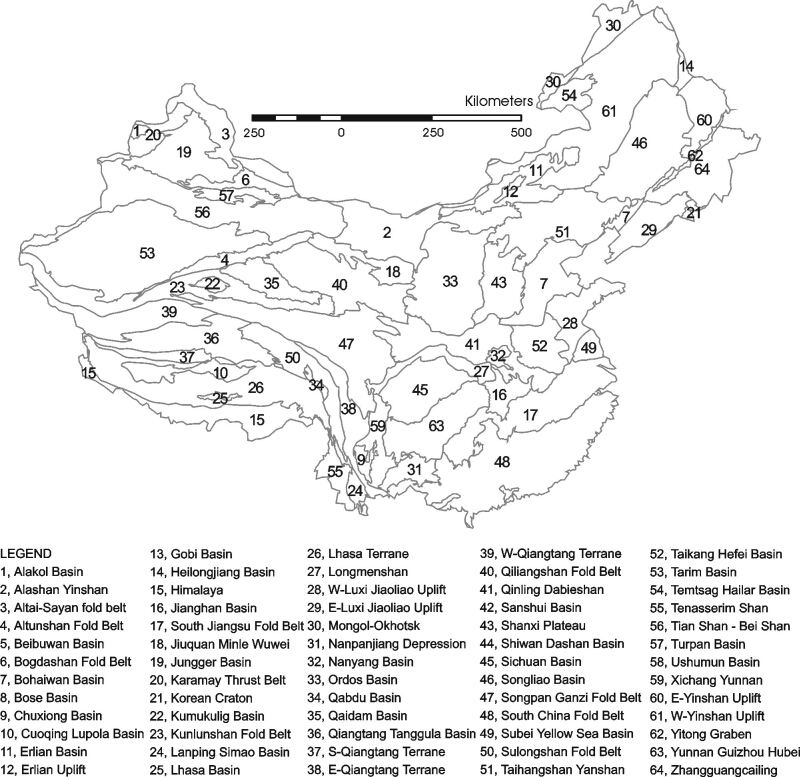
\includegraphics[width=1\textwidth]{chinazones.jpg}
   \caption{The tectonic map of China, based on USGS Open File Report 97-470C 
   (Wandrey and Low, 1998)}
   \label{fig:chinazones}
 \end{figure}

 With his  1963 paper, L.L. Sloss  was one of the  fathers of sequence
 stratigraphy, more than  a decade before this term  was introduced by
 Vail and Mitchum (1977). On the eve of the plate tectonic revolution,
 Sloss described cycles of  alternating sedimentation and erosion on a
 continental  (Sloss,  1960, 1963),  and  later  global (Sloss,  1976)
 scale. We  now know that these first-  and second-order stratigraphic
 cycles (Vail and Mitchum, 1977)  mainly are the result of the breakup
 and assemblage of super-continents, and of the related periodicity in
 the  rate of  ocean spreading  and the  volume of  mid-oceanic ridges
 (e.g.   Flemming and  Roberts,  1973). In  order  to reconstruct  the
 depositional  cycles, and  to correlate  them across  the continents,
 Sloss applied a  conceptually simple method, which is  similar to the
 one  that will  be used  in  this paper  for the  description of  the
 tectonic history of China.  Therefore,  I term it the "Sloss method".
 \\

 L.L. Sloss used isopach maps of  the United States, of Canada, and of
 the USSR to  calculate the preserved areal extent  and volume of each
 of the  stratigraphic units of  the maps.  Converting these  units to
 physical  time by  means of  the geological  time scale,  he obtained
 depositional time series, which he found to be remarkably similar for
 the  three areas  studied (Sloss,  1976).  Unfortunately,  no isopach
 atlas exists that  covers the entire territory of  China.  Instead, I
 use     the     digitized     geologic     and     tectonic     (Fig.
 \ref{fig:chinaslossSmallMagmatic})  map  at  a scale  of  1:5,000,000
 (USGS open  file reports 97-470F  and 97-470C). Although we  have the
 disadvantage  of poorer data  quality, we  also have  advantages that
 were  not   available  to  Sloss.   Computing   power  has  increased
 tremendously since  1976.  The tools of GIS  and statistical analysis
 prove to be very useful for our purposes.  \\

 \begin{landscape}
 \begin{figure}[p] \centering
 \centerline{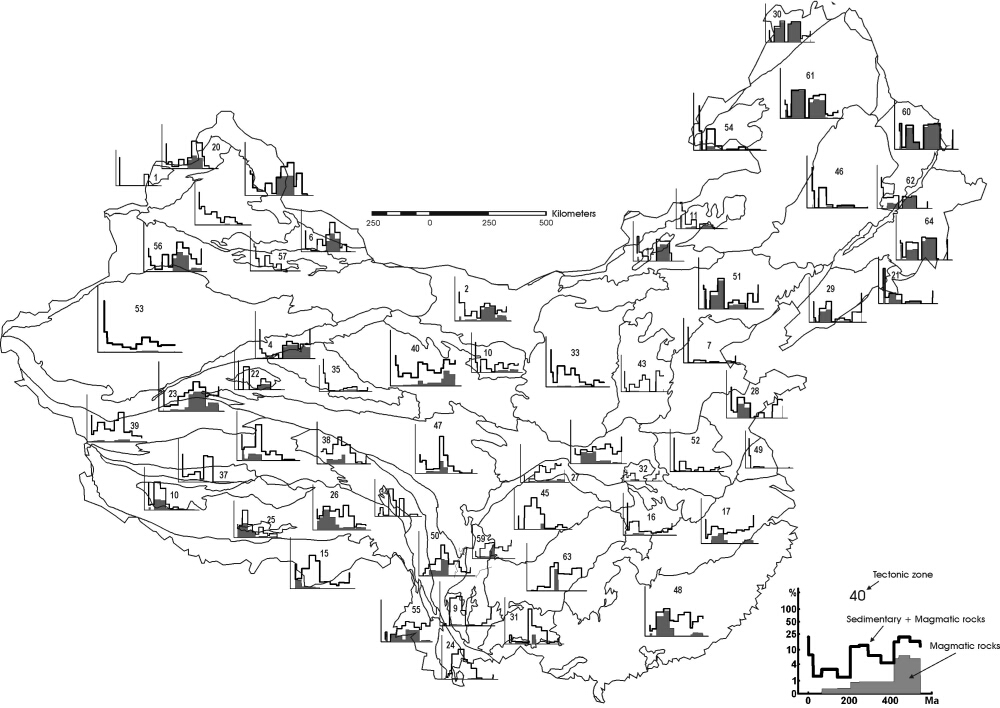
\includegraphics[width=1.2\textwidth]
   {chinaslossSmallMagmatic_n=1.jpg}}
 \caption{The "Sloss map" of continental China summarizes 
 both the  tectonic and  the geologic map.   The numbers  indicate the
 tectonic  zones, as  specified by  Fig.\ref{fig:chinazones}.  Some
 tectonic  zones  were  omitted  if   they  were  too  small  for  the
 calculation  of a  meaningful "Sloss  curve". In  each of  the "Sloss
 curves", the  black line represent  the percentage of the  total area
 (on a logarithmic scale) represented by  rocks of a certain age (on a
 linear  scale) in  the Phanerozoic.  The area  shaded grey  under the
 curve  represents  the  percentage  covered by  magmatic  rocks  (see
 inset).}
 \label{fig:chinaslossSmallMagmatic}
 \end{figure}
 \end{landscape}

 \section*{The Method} \label{sec:method}

 ~\indent For each of the tectonic  zones, the area covered by rocks of
 a certain  stratigraphic age  was calculated as  a percentage  of the
 total area  of the  tectonic zone.  Next,  these data  were converted
 into  time series  by means  of  the time  scale of  Harland {\it  et
 al.}(1990). The  time resolution of  the geologic map is  rather poor
 and not  uniform, with most units defined  at the chronostratigraphic
 systems level,  while some span as  much as an entire  era.  To solve
 this  problem, the  following  strategy was  used: given  overlapping
 stratigraphic units  1 and  2, of duration  S1 and  S2, respectively,
 $A^{S1}_{S2}$ is the areal contribution of  unit 2 to the part of the
 "Sloss curve" that overlaps in time with unit 1:

 \begin{equation}
   \label{eq:slossmethod}
     A^{S1}_{S2} = A^{S2}_{S2} \times \left( \frac{S1}{S2} \right)\\
 \end{equation}

 \noindent The use of equation       \ref{eq:slossmethod}      
 is  illustrated by  Fig.\ref{fig:slossmethod}.   We will  use it  for
 calculating  the  "Sloss  map"  of  China, which  is  shown  in  Fig.
 \ref{fig:chinaslossSmallMagmatic}.\\

 \begin{figure}[here]
 \begin{center}
 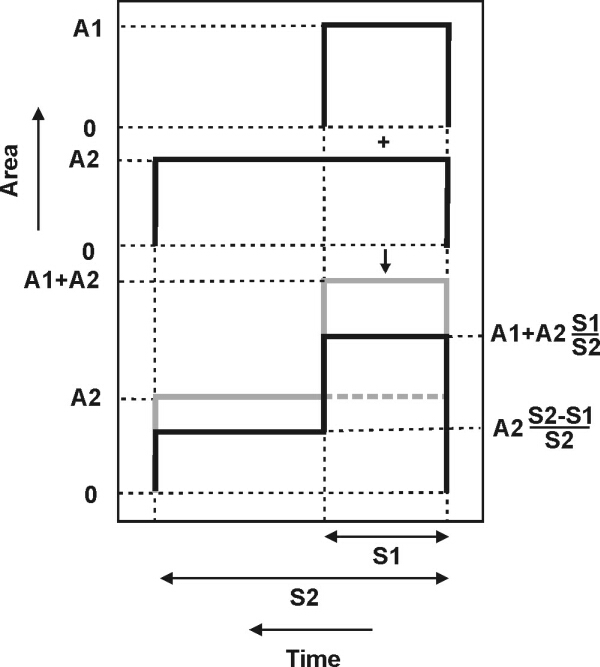
\includegraphics[width=0.6\textwidth]{slossmethod.jpg}
 \caption[fig:slossmethod]{If the total area of 
 the  geologic map that  is labeled  S1 is  A1, and  the stratigraphic
 subdivision named  S2 covers an  area A2, the corresponding  value of
 the "Sloss  curve" (black  curve, lowermost part  of the  figure) for
 each elementary  time step  (e.g. S1) is  a function of  the relative
 time overlap, and given by equation~\ref{eq:slossmethod} of the text.
 }\label{fig:slossmethod}
 \end{center}
 \end{figure}

 For the western United States, a  GIS version of the geologic map (at
 a  scale of 1:2,500,000)  is available,  in a  similar format  as the
 geologic map of China (King  and Beikman, 1974).  A "Sloss curve" was
 calculated for  a rectangular area,  located between 39$^o$N/100$^o$W
 and 49$^o$N/114$^o$W  and compared to  the curves that were  based on
 isopach maps for the same  area (Sloss, 1976).  Thus, the validity of
 the  above proposed  method could  be  tested.  The  results of  this
 exercise are shown on  Fig.\ref{fig:problems2}.  For reasons that are
 discussed  further  below,  the  fit  is  not  perfect.  Still,  most
 depositional  peaks  are located  at  the  same  times.  Taking  into
 account    these    remarks,   the    "Sloss    curves"   of    Figs.
 \ref{fig:chinaslossSmallMagmatic}  and \ref{fig:problems2} represents
 an important  simplification and abstraction of the  geologic map. We
 will use them to {\it compare} the different tectonic zones of China,
 and reconstruct their history.  Such analysis is reliable because all
 "Sloss curves" on  Fig.\ref{fig:chinaslossSmallMagmatic} are based on
 the same geologic map,  using the same stratigraphic subdivisions. It
 would be  more dangerous to make  inferences based on  a {\it single}
 "Sloss  curve", or  use the  method to  compare different  data sets,
 which    is    what    was    done   for    the    construction    of
 Fig.\ref{fig:problems2}.  Fig.\ref{fig:chinaslossSmallMagmatic} shows
 some interesting  and tectonically  meaningful features that  will be
 interpreted in the discussion section of this paper.\\

 \begin{figure}[here]
 \begin{center}
 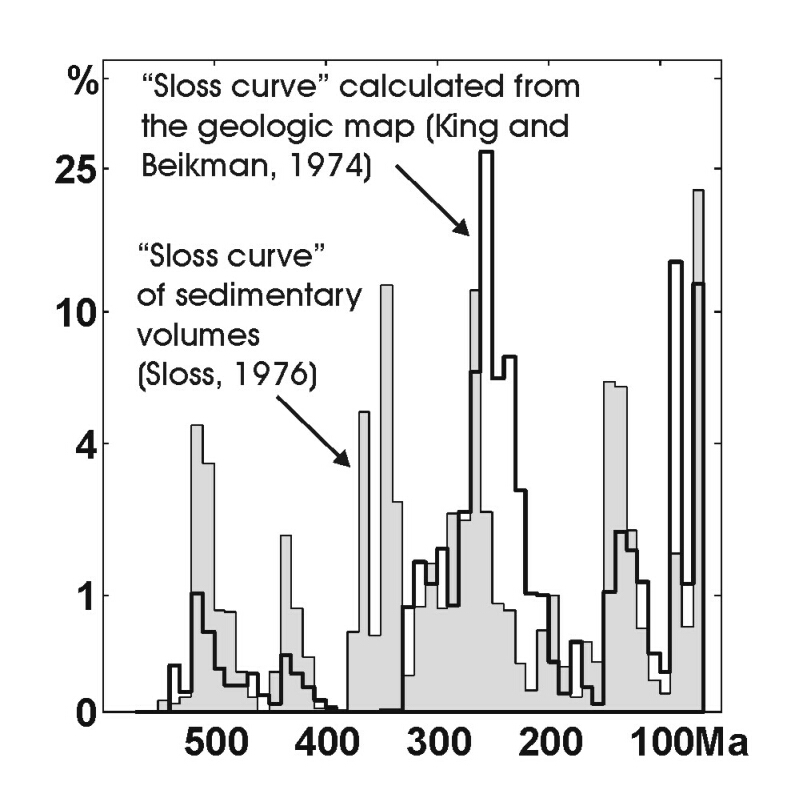
\includegraphics[width=0.6\textwidth]{problems2c.jpg}
 \caption{
 Comparison  of  the  "Sloss  curve"  of  the  western  United  States
 (rectangular area between  34$^o$N/100$^o$W and 49$^o$N/114$^o$W), as
 calculated  from  the geologic  map  (King  and Beikman,  1974)(black
 curve),  with the  curves of  sedimentary volume  published  by Sloss
 (1976) (gray  area) for  the same  area. Because  two  different data
 sources   were   used,  it   was   necessary   to  re-calculate   the
 "Sloss-curves"  for  identical  time  steps.  Not  surprisingly,  the
 height of  the peaks  differs between the  two curves in  most cases.
 This is  especially clear during  the Paleozoic, which  is especially
 affected by the "blanketing  effect". The important thing to remember
 about this figure is that the  major peaks and troughs are located at
 approximately the same times. Thus, the geologic map can be used as a
 proxy for the isopach map.}
 \label{fig:problems2}
 \end{center}
 \end{figure}

 \section*{Limitations and Uncertainties of the Method} 
 \label{sec:limitations}

 ~\indent The  most important problem  Sloss (1976) pointed out  in his
 method  was  the incompleteness  of  the  geologic record:  erosional
 processes progressively  remove greater fractions of  the rock record
 with time.  Because  the analysis that is presented  in this paper is
 not based  on isopach maps, but  on the geologic  map, these problems
 are aggravated and additional problems arise.  \\
 \begin {itemize}

 \item  First and  foremost, not  only erosional  processes,  but also
 sedimentary processes obscure the more distant geological past. It is
 possible  for  a  relatively  thin cover  of  horizontally  deposited
 sediments to completely dominate the geologic map of an area, even in
 cases  where  older  formations  represent much  larger  volumes  and
 thicknesses. This  "sedimentary blanketing effect"  is illustrated by
 Fig.~\ref{fig:problems1}. The  importance of the  "blanketing effect"
 dramatically   decreases  with   increasing  age.   Older  geological
 formations are more  likely to have been affected  by previous stages
 of  tectonism,  which  cause  folding and  tilting.  These  processes
 improve  the quality  of  outcrop  area as  a  proxy for  sedimentary
 thickness  and   volume  (Fig.\ref{fig:problems1}).   Therefore,  the
 "Sloss-like methodology" should be more reliable for the more distant
 past.  However, there  is a tradeoff with the  time resolution, which
 generally  {\it  decreases}  with   age.   The  Precambrian  is  only
 subdivided into  2 parts: Archean  and Proterozoic. For  this reason,
 the  Precambrian has  been  omitted from  the  map of  China in  Fig.
 \ref{fig:chinaslossSmallMagmatic}.  \\

 \item  Sloss included  lithological  data in  his  analysis. The  GIS
 version  of   the  geologic   map  of  China   distinguishes  between
 sedimentary  and   magmatic  rocks,   but  does  not   subdivide  the
 sedimentary  rocks.   Lithologies  obviously  can  provide  important
 information regarding the  tectonic setting of an area,  but they are
 less  easily   represented  by   numbers  that  can   be  objectively
 compared. Also  Sloss based his  conclusions mostly on  the numerical
 values      of      volume      and     preserved      area.       On
 Fig.\ref{fig:chinaslossSmallMagmatic},  the  area  under  the  "Sloss
 curves" covered by magmatic rocks is shaded gray.
 \end{itemize}

 \begin{figure}[here]
 \begin{center}
 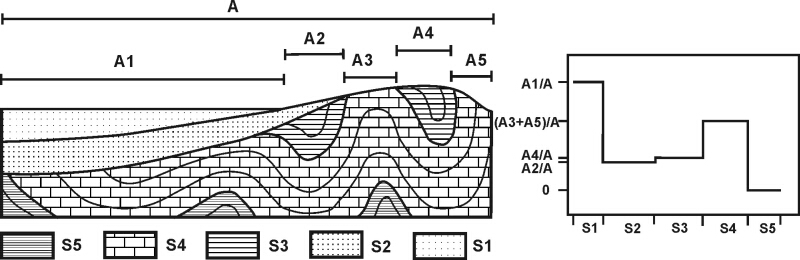
\includegraphics[width=1\textwidth]{problems1.jpg}
 \caption[fig:problems1]{Illustration of the sedimentary 
 "blanketing effect"  : steeply  tilted layers make  smaller outcrops,
 even though  they can  have greater thickness  and volume  than their
 sub-horizontal  sedimentary cover  ("blanket"). The  more  deformed a
 region is, the better the  geologic map, and its corresponding "Sloss
 curve",    represents   the    volumetric    distribution   of    the
 strata. }\label{fig:problems1}
 \end{center}
 \end{figure}

 \section*{Discussion: Tectonic History of China as Illustrated by its 
 "Sloss Map".} \label{sec:discussion}

 ~\indent Figure~\ref{fig:chinazones2} shows  how the 64 tectonic zones
 of  China  can   be  grouped  into  a  smaller   number  of  tectonic
 "regions".  This grouping  is in  close agreement  with  the tectonic
 zonation of  Zhang {\it et  al} (1984) and  Yin and Nie  (1996). This
 section   will  discuss   how   the  "Sloss   Map"   can  provide   a
 semi-independent     confirmation     of     its    validity.      On
 Fig.\ref{fig:chinazones2}, the  tectonic affinities are  indicated by
 different  hatching patterns.  The  hatching density  further divides
 the tectonic groups in subgroups  that are more convenient to discuss
 together.  It  is important to note  that some of  the tectonic zones
 were  assigned  to  a  tectonic  group in  a  rather  arbitrary  way.
 Generally, this is  the case for suture zones.  For example, the Tian
 Shan  was  considered as  part  of  the  "northern tectonic  region".
 However, we could also have put this range in the Tarim-Qaidam block,
 because  the Tian Shan  contains fragments  of both  tectonic groups.
 Similarly,  the Qinling-Dabie zone  was assigned  to the  North China
 block,  but being the  welding zone  with the  South China  block, it
 could  just as  well have  been made  part of  the latter.   The only
 "suture zone"  for which  an exception was  made is the  vast Songpan
 Ganzi  fold belt.   A special  discussion will  be dedicated  to this
 zone,  and  its relationship  with  the  surrounding tectonic  blocks
 (section dealing with Central China).

 \begin{figure}[htbp]
   \centering
   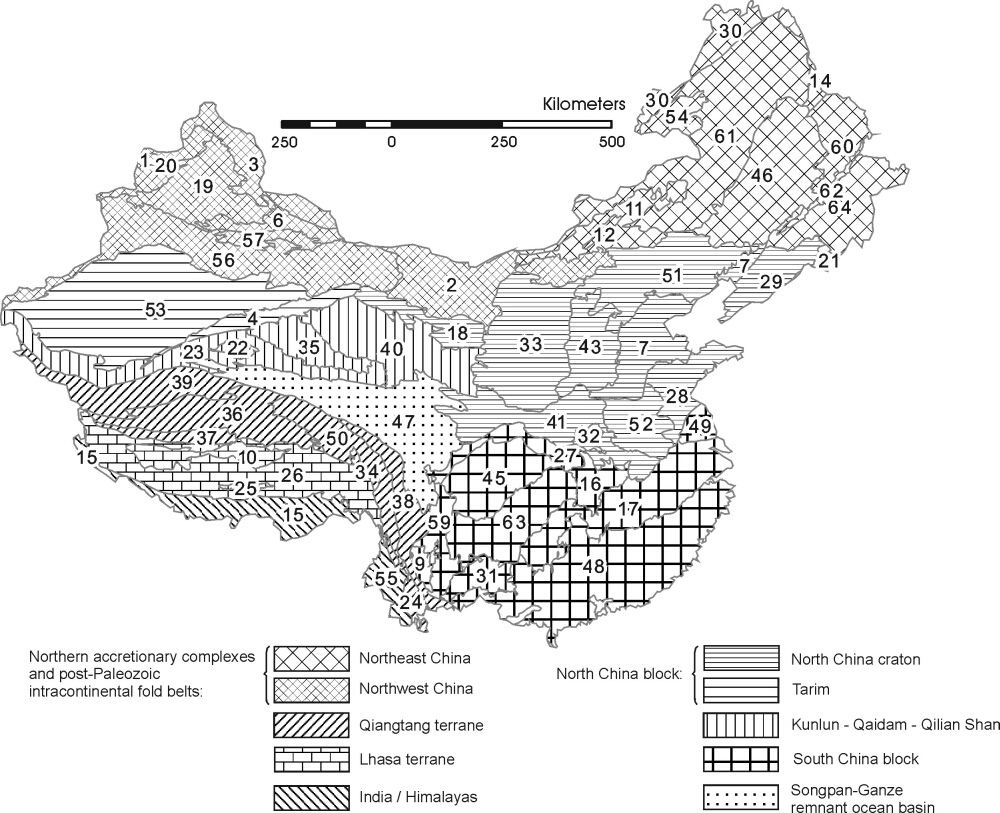
\includegraphics[width=1\textwidth]{chinazones2.jpg}
   \caption{The tectonic map of China, hatched according to 
 tectonic affinity.   Some tectonic groups are further  divided by the
 density  of the  hatching where  this facilitates  discussion  of the
 tectonic history in sections of the text.}
   \label{fig:chinazones2}
 \end{figure}

 \subsection*{Northern tectonic region} \label{sec:ntr}
 ~\indent  The  Northern  tectonic  region  consists  of  a  number  of
 microcontinents and early Paleozoic island arcs.  These were accreted
 to the  southern margin  of the Siberia-Kazakhstan  plate and  to the
 northern margin  of the Tarim-North  China block prior to  and during
 the final  collision between  these two, which  occured diachronously
 from the Carboniferous (west), until the Late Permian (east) (Yin and
 Nie,  1996).  The Northern  tectonic region  recorded changes  in the
 regional  tectonic  stress  field,  induced by  distant  accretionary
 events.  During the Mesozoic  and Cenozoic, Paleozoic fold belts were
 reactivated several times  as complicated systems of intracontinental
 mountain ranges and sedimentary  basins.  Although its tectonic zones
 have a  similar (Paleozoic)  tectonic history, the  Northern tectonic
 region is so  large, that we will continue  our discussion by further
 dividing it into an eastern and a western part.

 \subsubsection*{Northeast China} \label{sec:northeast}
 ~\indent Northeast  China is part  of the Mongolian  accretionary fold
 belt, which is a collage  of Ordovician to Early Permian island arcs,
 blueschist-bearing  assemblages, Paleozoic  ophiolites,  and possible
 microcontinental blocks  (Davis {\it  et al.}, 2001).   These tectonic
 settings stand out in the "Sloss curves" of Fig.  \ref{fig:northeast}
 by the  great relative importance of magmatic  lithologies, which are
 shaded  gray.  During  the  Late  Permian  and  Early  Triassic,  the
 Mongolian  arc terrane  was finally  welded together  with  the North
 China craton along  the Suolon suture (Yin and  Nie, 1996; Davis {\it
 et al.},  2001).  On the "Sloss  map", this event is  represented by a
 subsequent absence of deposits during the Triassic, which is probably
 due  to   the  compression   and  mountain  building   that  followed
 collision.    During   the    Late   Triassic,    the   controversial
 Mongolo-Okhotsk  ocean  opened to  the  north  of  the Mongolian  arc
 terrane. This ocean  started subducting both to the  north and to the
 south, causing a continued importance of magmatic rocks in the "Sloss
 curves" (figure~\ref{fig:northeast}) (Yin and Nie, 1996).  During the
 Jurassic and the Cretaceous, the Suolon suture was reactivated as the
 Yanshan fold  and thrust  belt, on the  northern margin of  the North
 China block (Davis {\it et  al}, 1998, 2001).  This will be discussed
 in more  detail later.   Important to  note here is  that one  of the
 hypotheses  for the  driving force  behind this  reactivation  is the
 Cretaceous  closure of the  Mongolo-Okhotsk ocean  (Zonenshain, 1990;
 Yin and Nie, 1996; Davis {\it et al.}, 1998, 2001).

 \begin{figure}[here]
 \begin{center}
 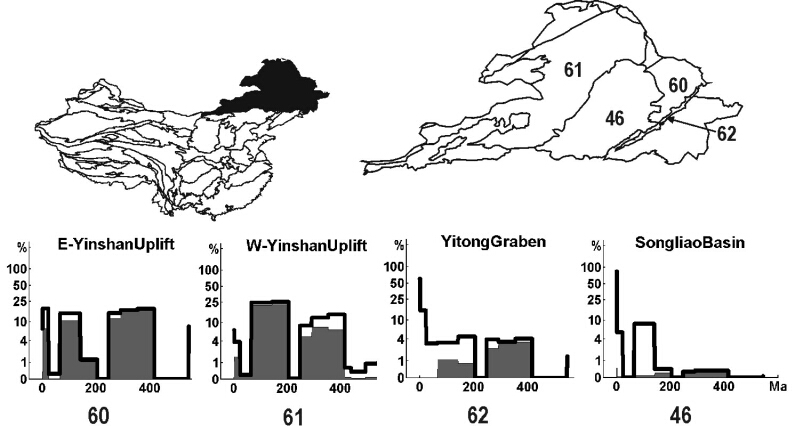
\includegraphics[width=0.8\textwidth]{northeasttris.jpg}
 \caption[fig:northeast]{ Northeast  China is  a tectonic  
  collage of accreted late Paleozoic terranes.  It is delimited to the
  south by the  Permo-Triassic Suolon suture, and to  the north by the
  Cretaceous  Mongolo-Okhotsk suture.   The  importance of  subduction
  processes during most of the  history of this region is reflected by
  the  large contribution  of magmatic  rocks to  the  "Sloss curves".
  During  the Mesozoic  large sedimentary  basins formed,  whereas the
  Suolon suture was reactivated south  of it, to form the Yanshan fold
  belt. The Paleogene is characterized by a dip in the "Sloss curves",
  except for the  Yitong graben, which indicates that  this feature is
  at least that old.  }\label{fig:northeast}
 \end{center}
 \end{figure}

 Alternatively,  also  the collisions  that  occured  on the  southern
 margin of  the Asian continent  (notably the Cretaceous  accretion of
 the  Lhasa  block),  could  have  been responsible  for  the  Yanshan
 compression (Graham {\it et  al}, 2001).  Curiously, this compression
 was also associated with basin-forming extension in the Mongolian arc
 terranes  (Davis  {\it et  al},  2001;  Graham  {\it et  al},  2001).
 Examples of such basins are  the Hailar basin and the Songliao basin,
 which  may have  been caused  by  Pacific back-arc  extension, or  by
 gravitational collapse  of the Late Paleozoic orogen  (Graham {\it et
 al}, 2001).  This apparent  paradox can be reconciled by partitioning
 of   the   Gobi   extensional   province   from   the   contractional
 Yinshan-Yanshan orogenic belt  by escape-tectonic strike-slip faults,
 such as the East Mongolian Zuunbayan fault, which would be associated
 with the coeval collisions  on the southern Asian and Mongolo-Okhotsk
 margins (Graham  {\it et al.},  2001).  During the Paleogene,  all the
 "Sloss  curves" of  Northeast  China show  a  dip, which  could be  a
 distant result  of the India-Eurasia collision,  or alternatively, be
 caused by changes  in the Pacific plate subduction  regime.  The only
 "Sloss   curve"  in   Northeast  China   that  does   show  Paleogene
 sedimentation  of  any  significance  is  the  Yitong  graben,  which
 suggests that this feature is at least that old (Tian and Du, 1987).

 \subsubsection*{Northwest China} \label{sec:northwest}
 ~\indent  The  pre-Devonian  history  of  Northwest  China  is  poorly
 understood.   Several microcontinents and  island arcs  were drifting
 around  on   the  subducting  Turkestan  ocean   that  separated  the
 Tarim-North  China  block  from Siberia-Kazakhstan  (Heubeck,  2001).
 Between the Early and  the Middle Devonian, southerly sourced clastic
 sediments  were deposited  along  the passive  continental margin  of
 North Tarim (Yin  and Nie, 1996).  These rocks  presently make up the
 southern Tian  Shan; thus  the latter does  not really belong  to the
 "Northern  tectonic  region".  During  the  Carboniferous,  two  more
 components of the  Tian Shan were welded to the  Tarim block: (1) the
 central Tian Shan block,  a microcontinent with Precambrian basement;
 and  then  (2)   the  northern  Tian  Shan  and   Junggar  blocks,  a
 post-Devonian arc terrane (Zhou {\it et al.}, 2001).  The collision of
 the Junggar arcs  and the Devonian Altai arcs with  the Tarim - North
 China block in the Carboniferous - Early Permian marked the beginning
 of the  diachronous closing of the Turkestan  ocean, which eventually
 led  to the  formation in  the northeast  of the  Permo-Triassic fold
 belt.  After its formation in  the Carboniferous, the Tian Shan, in a
 very similar way to  the Yinshan-Yanshan, would be reactivated during
 the Late Mesozoic  and the Late Cenozoic, as  a result of collisional
 events that  occured far to the  south of the range  (Dumitru {\it et
 al}, 2001).  Examples of such events are the Jurassic Qiangtang-Tarim
 collision and the Cretaceous Qiangtang-Lhasa collision.  Furthermore,
 the  Cenozoic   Himalaya  orogeny   has  caused  stresses   that  are
 transferred deep into the Asian continent.  They have made the modern
 Tian  Shan  the most  spectacular  of  all intracontinental  mountain
 belts, with elevations of up to 7,400m, at more than 1,000km from the
 suture zone (Molnar and Tapponnier, 1975).

 \begin{figure}[here]
 \begin{center}
 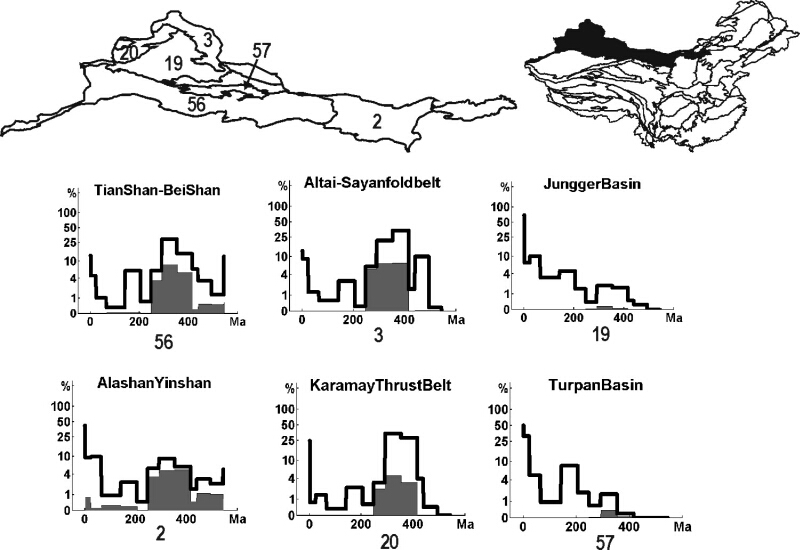
\includegraphics[width=0.8\textwidth]{northwesttris.jpg}
 \caption{
 Very similar to Northeast China,  Northwest China also is composed of
 a  number of  microcontinents  and island  arcs,  that were  accreted
 during  the Paleozoic.   Magmatic rocks  dominate the  "Sloss curves"
 until  the Carboniferous-Permian,  which corresponds  with  the final
 closure of  the Turkestan  ocean and the  formation of  the ancestral
 Tian Shan. In  contrast with the Northeast (Fig.\ref{fig:northeast}),
 there is no post-Paleozoic magmatism.  The "Sloss curves" of the fold
 belts all show a Triassic dip, a Jurassic high, a Cretaceous dip, and
 a  Cenozoic high.  These reflect  the repeated  reactivation  of this
 region due to ongoing collisions  on the southern margin of the Asian
 continent.  }\label{fig:northwest}
 \end{center}
 \end{figure}

 The  "Sloss   curves"  of  different  portions   of  Northwest  China
 (Fig.\ref{fig:northwest})  share numerous  characteristics  with each
 other, indicating a common  tectonic history since the Carboniferous.
 The   Late  Paleozoic   is  characterized   by   voluminous  magmatic
 lithologies,  which represents  the subduction  dominated  setting of
 many  of  the  terranes  of  this area.   From  the  Permian  onward,
 magmatism  ceased, in  marked  contrast with  the  tectonic zones  of
 northeastern China.   Indeed, in the  northeast the existence  of the
 Mongolo-Okhotsk ocean,  and the  proximity to the  subducting Pacific
 Ocean,  continued  to generate  magmas  throughout  the Mesozoic  and
 Cenozoic,  which  was not  the  case  for  northwest China.   Another
 characteristic of most zones of the "Sloss map" of Northwest China is
 a pronounced  dip during the  Triassic, which was probably  caused by
 mountain building that followed  closure of the Turkestan ocean, with
 the addition  of the compressional  stresses caused by  the southerly
 Qiangtang-Tarim collision.  The  Jurassic shows up as a  peak in most
 "Sloss  curves".   This   could  represent  post-orogenic  subsidence
 ("collapse"). The  Cretaceous is a  dip again, corresponding  to Late
 Mesozoic reactivation of the Tian  Shan that is detected by a cluster
 of Cretaceous apatite  fission track ages (Bullen {\it  et al.}, 2001;
 Dumitru  {\it et  al}, 2001).   Finally, the  Cenozoic  "Sloss curve"
 shows an  increase. This is  caused by a strong  "blanketing effect",
 and reflects  the formation of  large foreland basins  (e.g, Junggar,
 Turpan) between the different mountain ranges (e.g., Tian Shan, Bogda
 Shan).   The  structural   and  stratigraphic  relief  between  these
 coexisting tectonic elements can  attain several thousand meters over
 distances of just a few tens of kilometers.

 \subsection*{North China Block} \label{sec:ncb}
 ~\indent  The  Tarim  block  and  the North  China  craton  are  often
 postulated to have behaved as  a single tectonic block since at least
 the  early Paleozoic (e.g.   Zhang {\it  et al.},  1984; Yin  and Nie,
 1996).  Others  have suggested that  they were separate  blocks until
 the Permo-Triassic  closure of the Turkestan ocean  (Zhou and Graham,
 1996a; Yang {\it  et al.}, 1997).  That the Tarim  block and the North
 China  craton  are only  connected  by  a  very narrow  strip.   This
 "problem" is  solved by restoring $\sim$ 400km  of Cenozoic sinistral
 displacement  along  a  controversial Altyn  Tagh-Alxa-East  Mongolia
 fault (Yue and Liou, 1999; Yue  {\it et al.}, 2001).  In this section,
 we will discuss the North  China craton {\it sensu stricto}, which is
 the eastern  part of  the North China-Tarim  block.  The  North China
 craton is bordered to the  north by the Permo-Triassic Suolon suture,
 which   was  reactivated   during   the  Jurassic   as  the   Yanshan
 intracontinental fold belt  (Davis {\it et al.}, 1998,  2001).  To the
 southwest, the North China craton is sutured against the Qaidam block
 along  the Qilian  Shan;  the  suture marks  a  collisional event  of
 Devonian age.  Due east of the Qilian Shan is the Qinling-Dabie Shan,
 which  represents the  Permo-Triassic  collision of  the North  China
 block with the South China block (Yin and Nie, 1996; Zhou and Graham,
 1996b).  To  the southeast,  the North China  block is offset  by the
 sinistral Tan Lu fault system.\\

 Although named a "craton" (it  has Archean basement), the North China
 tectonic  group underwent substantial  internal deformation  over the
 course of its  Phanerozoic history.  The "Sloss curves"  of the North
 China craton do  not tell a simple story.   Important information has
 been obscured by the "blanketing effect". This is especially the case
 for the  Cenozoic Bohai rift  basin.  During the Late  Triassic, this
 zone  roughly corresponded  to the  "Huabei plateau",  which  was the
 result of  continuing convergence after the collision  of South China
 with North  China (Yin and  Nie, 1996).  Sediments derived  from this
 topographic high  were deposited in the neighboring  Shanxi and Ordos
 basins, where they are responsible  for a Triassic peak in the "Sloss
 curves". This is a feature that will be seen more often in the "Sloss
 map" of central China (discussed below; Fig.\ref{fig:central}).

 \subsection*{South China block} \label{sec:south}
 ~\indent The  South China  block is a  relatively stable  craton (also
 called the "Yangtze craton") that has a relatively insensitive "Sloss
 curve". In the Jiangsu- and South China fold belts, all stratigraphic
 ages are represented  approximately to an equal degree,  with a small
 preference  to the Quaternary  due to  the "blanketing  effect".  The
 "Sloss curves" of the western  part of the South China tectonic group
 show a  distinct peak in the  Triassic.  This marks  the collision of
 the  South  China  block with  the  North  China  block, as  will  be
 discussed below.

 \subsection*{Tarim-Qaidam} \label{sec:tarimqaidam}
 ~\indent  As  was  previously  discussed, disagreement  exists  as  to
 whether  or not  the  Tarim block  and  the North  China craton  were
 separate tectonic entities before the Permian.  A similar controversy
 exists about the Qaidam block.   Some have suggested that it was part
 of the  Tarim before being  cut off and  displaced by the  Altyn Tagh
 fault (Zhou  and Graham 1996a; some  extent also Yin  and Nie, 1996),
 whereas  others think  that the  two to  represent  separate tectonic
 blocks (e.g.  Zhang {\it  et al.}, 1984).   The discovery of  a Middle
 Paleozoic suture  zone in the Altyn  Tagh favors the  latter point of
 view (Sobel and Arnaud, 1999). After the Qaidam and Tarim blocks were
 welded  together, an  extensive, continuous,  late Paleozoic  - early
 Mesozoic   Kunlun  magmatic  arc   developed  along   their  southern
 margin.  This   arc  died  during  the  Triassic   collision  of  the
 Tarim-Qaidam block with the Qiangtang block.\\

 The closure of the ocean  basin that existed between the Tarim-Qaidam
 block and the Qiangtang block, is  marked by the abrupt ending of the
 (gray-shaded)  magmatic area under  the "Sloss  curve" of  the Kunlun
 tectonic zone. The  same is true for the  Altun Shan, where magmatism
 ended with  the closure of the  ocean that existed  between Tarim and
 Qaidam. Due to the "blanketing  effect", little can be said about the
 "Sloss curves"  of the  Qaidam and Tarim  basins themselves.  In this
 case, it  would be  particularly valuable to  have access  to isopach
 maps such as the ones Sloss (1976) used.

 \subsection*{Central China, Songpan Ganzi, and the 
 Permian-Triassic  N-China/S-China collision} \label{sec:songpanganze}
 ~\indent The  most representative tectonic element for  this region is
 the Songpan-Ganzi fold belt.   This tectonic zone is characterized by
 a     striking     depositional      peak     in     the     Triassic
 (Fig.\ref{fig:central}).  This peak can  be recognized  slightly less
 spectacularly in the zones  immediately to the south of Songpan-Ganzi
 (e.g., the  Sichuan Basin, Sulong  Shan). Sloss (1963, 1976)  was not
 the  first  person to  recognize  that the  Triassic  was  a lull  in
 continental  sedimentation.  It followed  immediately after  the last
 (Variscan) stages of the assemblage of the Pangea supercontinent, and
 is  characterized by  very low  global sea  level (Vail  and Mitchum,
 1977).   Hence, the abundance  of Triassic  deposits in  the tectonic
 zones  of   Central  China   must  indicate  an   important  tectonic
 event. This event is the  diachronous suturing of the North and South
 China blocks (Zhou and  Graham, 1996b). North of Songpan-Ganzi (e.g.,
 Altun  Shan), the  Triassic shows  up as  a low  point in  the "Sloss
 curve". This  could either be the  result of the  worldwide sea level
 drop described above  or alternatively, be caused by  the same events
 that caused the Triassic peak  in and south of Songpan-Ganzi. Indeed,
 if the Triassic orogeny was the result of northward underthrusting of
 the South  China block under the  North China block,  it seems likely
 that the  zones north of the  suture zone would  be uplifted, whereas
 the southern zones would flexurally subside. A modern day analogue to
 this would  be the  association on either  side of  the Indus-Tsangpo
 suture  zone of  the  North  Indian Ganges  foreland  basin, and  the
 Tibet-Qinghai Plateau.

 \begin{figure}[here]
 \begin{center}
 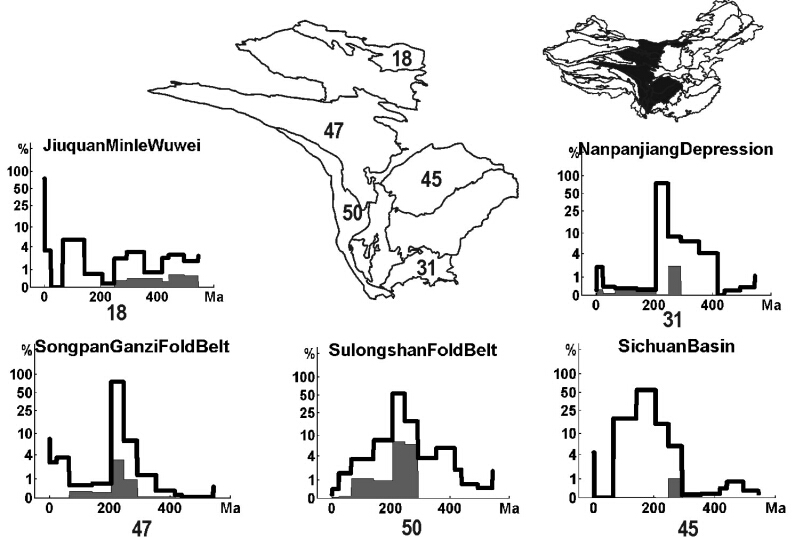
\includegraphics[width=0.8\textwidth]{centraltris.jpg}
 \caption{
 The "Sloss map" of Central  China shows a very characteristic peak of
 sedimentation and  magmatism in the  Triassic for the  tectonic zones
 south  of the  Songpan Ganzi  complex.  This  peak is  caused  by the
 diachronous collision between the  North China and South China blocks
 (Zhou and  Graham, 1996). The zones  north of the suture  zone show a
 lack  of sedimentation  at the  same  time, possibly  related to  the
 uplift   and    compression   caused   by    continental   collision.
 }\label{fig:central}
 \end{center}
 \end{figure}

 \subsection*{Southwestern China} \label{sec:southwest}
 ~\indent  The Qiangtang  block  drifted off  from  Gondwana some  time
 during the Paleozoic (Yin  and Harrison, 2000).  During the Triassic,
 the  ocean  that  separated  the  Qiangtang terrane  from  the  Asian
 continent started  subducting beneath it. The northern  margin of the
 Qiangtang  terrane became  an active  one, which  is reflected  in an
 increase   of   the   magmatic   area  under   its   "Sloss   curves"
 (Fig.~\ref{fig:southwest}).    Almost   immediately   following   the
 Permo-Triassic  collision  of  South  China  with  North  China,  the
 Qiangtang-Indochina block was  underthrusted by the amalgamated South
 China and Qaidam-Tarim blocks along  the Jinsha suture (Chang {\it et
 al},  1986;  Yin  and  Nie,  1996;  Yin  and  Harrison,  2000).   The
 Songpan-Ganzi remnant ocean basin was trapped in the triangular space
 between  the three aforementioned  blocks. The  Triassic peak  in the
 "Sloss  curves"  of  the   Qiangtang  block  testify  of  this  event
 (Figs.\ref{fig:central}      and~\ref{fig:southwest}).       Although
 subduction-related magmatism  stopped in the Kunlun,  it continued in
 the Qiangtang  block, along with the  approach from the  south of the
 Gondwana-derived  Lhasa  block. The  Lhasa  block  collided with  the
 Qiangtang  block   along  the  Banggong-Nujiang   suture  during  the
 Cretaceous (All\`egre {\it et al.}, 1984; Dewey {\it et al.}, 1988; Yin
 and Nie,  1996; Yin and Harrisson, 2000).   Whereas the underthrusted
 Qiangtang block was  deformed and uplifted (marked by  a relative low
 in  its "Sloss  curves"),  the underthrusting  Lhasa block  underwent
 flexural subsidence and is generally characterized by a "Sloss peak".
 After the collision of the  Lhasa block with the Qiangtang block, the
 oceanic  crust  that  separated  the  Lhasa  block  from  the  Indian
 subcontinent  subducted beneath  the Lhasa  block, which  resulted in
 extensive  magmatic  activity and  the  development  of the  Gangdese
 batholith (All\`egre {\it et al.},  1984; Yin and Harrison, 2000).  At
 approximately  45Ma,  India  finally  collided with  Asia  along  the
 Indus-Tsangpo suture (Le  Pichon {\it et al.}, 1992).  This led to the
 intensely studied, but poorly understood Himalaya-Tibet orogeny.  The
 Tibet-Qinghai Plateau  is believed to have resulted  mainly from this
 final collision,  although it has been suggested  that a pre-existing
 plateau formed  after the Kunlun-Qiangtang collision  (Murphy {\it et
 al}, 1997). The present day Tibet-Qinghai Plateau comprises the Lhasa
 terrane,   the   Qiangtang   terrane,   and  to   some   extent   the
 Kunlun-Qaidam-Qilian  Shan tectonic  group.   At the  same time,  the
 Himalaya-Tibet  orogeny reactivated  many of  the tectonic  zones and
 groups that have  been discussed in previous paragraphs.  This is the
 case for  the Tian Shan and the  Altai, but also for  the Altun Shan,
 which appear  to have  acted as  a zone of  weakness that  became the
 preferred  locus  for  the  continental-scale  Altyn  Tagh  sinistral
 strike-slip  fault.  The  Kunlun, Xianshui-He,  and Red  River faults
 roughly  follow the  Kunlun-Anyemaqen,  Jinsha, and  Banggong-Nujiang
 sutures, respectively  (Tapponnier {\it  et al.}, 2001).   Thus, fault
 reactivation seems  to be  a major factor  in the deformation  of the
 Chinese tectonic  "jigsaw puzzle".  The translation of  this in terms
 of  "Sloss curves" is  a trivial  one: topographic  depressions cause
 Cenozoic  peaks, whereas  areas  of high  relief  show a  dip in  the
 Cenozoic "Sloss curve". These signatures  can be seen all over China,
 and perhaps  even affect  the Pacific margin  (e.g.  Jolivet  {\it et
 al}, 1990).

 \begin{figure}[here]
 \begin{center}
 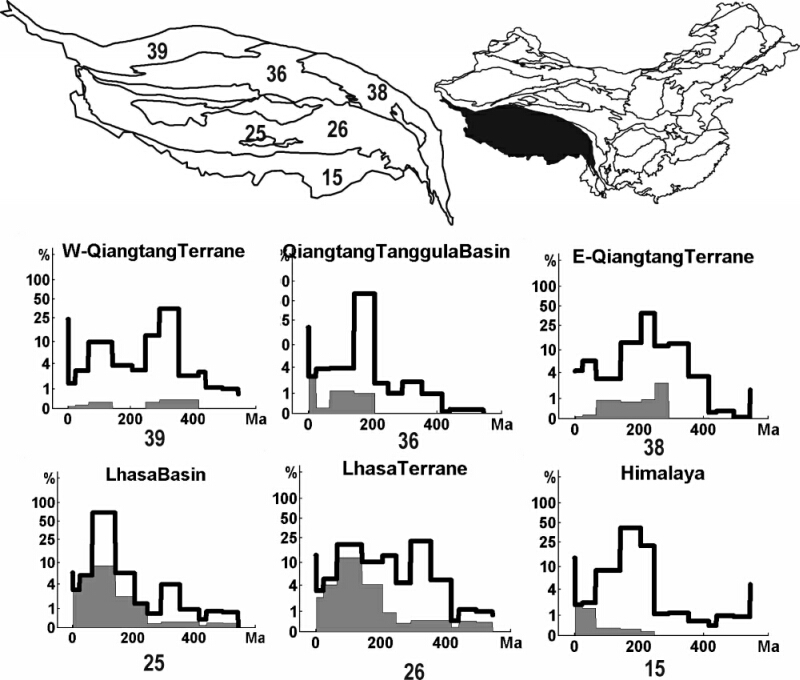
\includegraphics[width=0.8\textwidth]{southwestbisb.jpg}
 \caption{ 
 The Tibet  Plateau consists of  three tectonic blocks:  the Qiantang,
 Lhasa, and India blocks.  Qiangtang underthrusted the Kunlun block in
 the Late  Triassic, which shows  up as a  peak in its  "Sloss curve".
 Subsequently,  the Lhasa  block  collided with  the Qiangtang  block,
 after  the closure of  an oceanic  basin that  was associated  with a
 magmatic   arc  and   a  substantial   of  gray   under   the  "Sloss
 curve". Finally,  the southern  margin of the  Lhasa block  became an
 active  one  (represented  by  a  predominantly  gray  shaded  "Sloss
 curve"), until the final collision  with India, which caused a dip in
 the  Cenozoic curves  of  both  the Qiangtang  and  the Lhasa  block.
 }\label{fig:southwest}
 \end{center}
 \end{figure}

 \section*{Conclusions} \label{sec:conclusion}

 ~\indent I have developed  a method for representing a two-dimensional
 geologic map  by a one-dimensional depositional  time series, similar
 to the way  L.L.Sloss represented the geologic maps  of North America
 and  eastern  Europe (Sloss,  1976).   Going  one  step further,  the
 geologic  map and  the tectonic  map of  China were  united  into one
 "Sloss map".  Despite limitations and assumptions of  the method, the
 "Sloss map" proves useful for recognizing the most important tectonic
 events  of Phanerozoic  China, and  for delimiting  tectonic regions,
 which  can comprise  multiple tectonic  zones.   The Permian-Triassic
 North China - South China  collision and the Cenozoic India - Eurasia
 collision  stand out  especially clearly.   Also,  difference between
 stable  cratons  and tectonically  more  sensitive accretionary  fold
 belts can easily be recognized.  \\

 Major improvements  could be made  with the incorporation  of isopach
 maps, rather than ordinary geologic maps. Other welcome changes would
 be increased  time resolution, and the addition  of more lithological
 parameters  to  the  geologic  map.  If  all  these  conditions  were
 fulfilled, it might be  possible to fully automate the interpretation
 of the "Sloss map" by means of a statistical correlation analysis. If
 extended to other continents, the  "Sloss analysis" could prove to be
 as useful in tracing and  describing the {\it breakup} of continents,
 as it is with continental  {\it accretion}, which I have demonstrated
 in this paper with China's history of amalgamation.  The first places
 to examine in  the case of China would be  Gondwana, and the southern
 margin  of  the Tethys.   Indeed,  most  of  the tectonic  blocks  of
 Fig.\ref{fig:chinaslossSmallMagmatic}  originally  drifted  off  from
 continental areas now consituting India and Australia (\c{S}eng\"{o}r
 and Natal'in,  1996). The methodology  described in this  paper might
 prove to be a good first-order way of detecting such associations.\\

 Another application of  the "Sloss method" in its  present form would
 be the study  of orogenic terranes.  If geologic maps  exist in a GIS
 form, the "Sloss  curve" derived from the geologic  map could be used
 as   a   proxy  for   the   isopach   map,   as  was   suggested   in
 Fig.\ref{fig:problems2}.   Doing  this   may  yield  insight  in  the
 evolution of rates  of deposition until the time  of collision, which
 is important for understanding the mechanisms of mountain building.

 \section*{Acknowledgements}

 Many thanks to Steve Graham for useful suggestions and encouragement,
 and to Stanford University for financial support.

 \section*{References Cited}

 \begin{description}

 \item  All\`egre, C. J.,  Courtillot, V.,  Tapponnier, P.,  Hirn, A.,
 Mattauer, M., Coulon,  C., Jaeger, J. J., Achache,  J., Schaerer, U.,
 Marcoux, J.,  Burg, J.  P., Girardeau, J.,  Armijo, R.,  Gariepy, C.,
 Goepel, C.,  Li, T., Xiao, X., Chang,  C., Li, G., Lin,  B., Teng Ji,
 W., Wang, N.,  Chen, G., Han, T., Wang, X., Den,  W., Sheng, H., Cao,
 Y., Zhou,  J., Qiu, H.,  Bao, P., Wang,  S., Wang, B., Zhou,  Y., and
 Ronghua,  X., 1984,  Structure  and evolution  of the  Himalaya-Tibet
 orogenic belt: Nature, v. 307, no. 5946, p. 17-22.\\

 \item Bullen, M. E., Burbank, D. W., Garver, J. I., and Abdrakhmatov,
 K.  Y., 2001, Late  Cenozoic tectonic  evolution of  the northwestern
 Tien Shan; new age estimates for the initiation of mountain building:
 Geological   Society   of  America   Bulletin,   v.   113,  no.   12,
 p. 1544-1559.\\

 \item Chang,  C., Chen, N.,  Coward, M. P.,  Deng, W., Dewey,  J. F.,
 Gansser,  A., Harris,  N. B.  W., Jin,  C., Kidd,  W. S.  F., Leeder,
 M. R., Li, H.,  Lin, J., Liu, C., Mei, H., Molnar,  P., Pan, Y., Pan,
 Y., Pearce,  J. A., Shackleton, R.  M., Smith, A. B.,  Sun, Y., Ward,
 M.,  Watts, D. R.,  Xu, J.,  Xu, R.,  Yin, J.,  and Zhang,  Y., 1986,
 Preliminary conclusions of the Royal Society and Academia Sinica 1985
 geotraverse of Tibet: Nature, v. 323, no. 6088, p. 501-507.\\

 \item Davis,  G. A., Cong, W.,  Zheng, Y., Zhang, J.,  Zhang, C., and
 Gehrels, G.  E., 1998, The enigmatic Yinshan  fold-and-thrust belt of
 northern  China; new  views on  its intraplate  contractional styles:
 Geology, v. 26, no. 1, p. 43-46.\\

 \item Davis, G. A., Zheng, Y., Wang, C., Darby, B. J., Zhang, C., and
 Gehrels, G.,  2001, Mesozoic tectonic  evolution of the  Yanshan fold
 and  thrust belt,  with emphasis  on Hebei  and  Lianoning provinces,
 northern  China: Memoir  -  Geological Society  of  America, v.  194,
 p. 171-197.\\

 \item Dewey, J.  F., Shackleton, R. M., Chang, C.,  Sun, Y., and Yin,
 J., 1988,  The tectonic evolution of the  Tibetan Plateau [Monograph]
 The geological evolution of Tibet; report of the 1985 Royal Society -
 Academia   Sinica   geotraverse   of  the   Qinghai-Xizang   Plateau:
 Philosophical Transactions of the  Royal Society of London, Series A:
 Mathematical and Physical Sciences, v. 327, no. 1594, p. 379-413.\\

 \item Dumitru, T. A., Zhou, D., Chang, E. Z., Graham, S. A., Hendrix,
 M. S.,  Sobel, E. R., and  Carroll, A. R.,  2001, Uplift, exhumation,
 and deformation in the Chinese Tian Shan: Memoir - Geological Society
 of America, v. 194, p. 71-99.\\

 \item  Flemming,  N.C.,  and  Roberts, D.G.,  1973,  Tectono-eustatic
 Changes in Sea Level and Seafloor Spreading: Nature (London), v. 243,
 p. 19-22.\\

 \item Graham, S. A., Hendrix,  M. S., Johnson, C. L., Badamgarav, D.,
 Badarch, G.,  Amory, J., Porter, M.,  Barsbold, R., Webb,  L. E., and
 Hacker, B. R., 2001,  Sedimentary record and tectonic implications of
 Mesozoic rifting in Southeast Mongolia: Geological Society of America
 Bulletin, v. 113, no. 12, p. 1560-1579.

 \item Harland, W.B., Armstrong, R.L., Cox, A.V., Craigh, L.E., Smith,
 A.G., and Smith, D.G., 1990,  A Geologic time scale 1989: Cambridge ;
 New York, Cambridge University Press, xvi, 263 p.\\

 \item Hendrix,  M.S., and Davis,  G.A., 2001, Paleozoic  and Mesozoic
 tectonic  evolution of central  Asia :  from continental  assembly to
 intracontinental deformation:  Boulder, Colo., Geological  Society of
 America, vi, 447 p.\\

 \item Heubeck, C.,  2001, Assembly of Central Asia  during the middle
 and late Paleozoic:  Memoir - Geological Society of  America, v. 194,
 p. 1-22.\\

 \item  Jolivet, L., Davy,  P., and  Cobbold, P.,  1990, Right-lateral
 shear  along  the  Northwest  Pacific margin  and  the  India-Eurasia
 collision: Tectonics, v. 9, no. 6, p. 1409-1419.\\

 \item King, P.B., and Beikman, H.M., 1974, Geologic map of the United
 States  (exclusive of  Alaska and  Hawaii), U.  S.  Geological Survey
 Reston VA United  States (USA), available in digital  format as: USGS
 Digital Data Series DDS-11.\\

 \item Le Pichon, X., Fournier, M., and Jolivet, L., 1992, Kinematics,
 topography, shortening, and extrusion in the India-Eurasia collision:
 Tectonics, v. 11, no. 6, p. 1085-1098.\\

 \item  Molnar, P., and  Tapponnier, P.,  1975, Cenozoic  tectonics of
 Asia; effects of a continental  collision: Science, v. 189, no. 4201,
 p. 419-426.\\

 \item Murphy,  M. A., Yin, A.,  Harrison, T. M., Duerr,  S. B., Chen,
 Z., Ryerson, F. J., Kidd, W. S. F., Wang, X., and Zhou, X., 1997, Did
 the Indo-Asian collision alone  create the Tibetan Plateau?: Geology,
 v. 25, no. 8, p. 719-722.\\

 \item   \c{S}eng\"{o}r,    A.M.C.,   and   Natal'in,    B.A.,   1996,
 Paleotectonics of  Asia: fragments  of a synthesis,  in Yin,  A., and
 Harrison,  T.M.,  eds., The  Tectonic  evolution  of Asia:  Cambridge
 [England] ; New York, Cambridge University Press, p. 486-640.\\

 \item Sobel, E. R., and Arnaud, N., 1999, A possible middle Paleozoic
 suture  in  the  Altyn Tagh,  NW  China:  Tectonics,  v. 18,  no.  1,
 p. 64-74.\\

 \item    Sloss,   L.L.,   1960,    Interregional   time-stratigraphic
 correlation:   Geological  Society  of   America  Bulletin,   v.  71,
 p. 1976.\\

 \item Sloss, L.L., 1963, Sequences  in the cratonic interior of North
 America: Geological Society of America Bulletin, v. 74, p. 93-113.\\

 \item  Sloss, L.L., 1976,  Areas and  volumes of  cratonic sediments,
 western   North  America   and   eastern  Europe:   Geology,  v.   4,
 p. 272-276.\\

 \item Steinshouer,  D.W., Qiang, J.,  McCabe, P.J., and  Ryder, R.T.,
 1998,  Maps  showing  geology,  oil  and  gas  fields,  and  geologic
 provinces  of   the  Asia  Pacific  Region,   USGS  Open-File  Report
 97-470F.\\

 \item  Tapponnier, P.,  Xu, Z.,  Roger,  F., Meyer,  B., Arnaud,  N.,
 Wittlinger, G., and Yang, J.,  2001, Oblique stepwise rise and growth
 of the Tibet Plateau: Science, v. 294, no. 5547, p. 1671-1677.\\

 \item  Tian, Z., and  Du, Y.,  1987, Formation  and evolution  of the
 Yilan-Yitong  Graben, in  Froidevaux, C.,  and Tan  Tjong,  K., eds.,
 Tectonophysics: Amsterdam, Elsevier, p. 165-173.\\

 \item Vail, P.R., and  Mitchum, R.M., Jr., 1977, Seismic stratigraphy
 and global changes of sea level; Part 1, Overview [Monograph] Seismic
 stratigraphy; applications to hydrocarbon exploration.\\

 \item Wandrey, C.J.,  and Law, B.E., 1998, Maps  showing geology, oil
 and gas fields  and geologic provinces of South  Asia, USGS Open-File
 Report 97-470C.\\

 \item Yang, Z.,  Zhou, D., and Graham, S. A.,  1997, Extrusion of the
 Altyn  Tagh wedge; a  kinematic model  for the  Altyn Tagh  Fault and
 palinspastic reconstruction of  northern China; discussion and reply:
 Geology, v. 25, no. 5, p. 475-477.\\

 \item  Yin,  A.,  and  Nie,  S.,  1996,  A  Phanerozoic  palinspastic
 reconstruction of China and its  neighboring regions, in Yin, A., and
 Harrison,  T. M.,  eds., The  Tectonic evolution  of  Asia: Cambridge
 [England] ; New York, Cambridge University Press, p. 442-485.\\

 \item Yin,  A., and Harrison,  T.M., 2000, Geologic evolution  of the
 Himalayan-Tibetan  orogen:  Annual  Review  of  Earth  and  Planetary
 Sciences, v. 28, p. 211-280.\\

 \item Yue, Y.,  and Liou, J. G., 1999,  Two-stage evolution model for
 the Altyn Tagh Fault, China: Geology, v. 27, no. 3, p. 227-230.\\

 \item  Yue,  Y., Liou,  J.-G.,  and  Graham,  S. A.,  2001,  Tectonic
 correlation   of  Beishan   and  Inner   Mongolia  orogens   and  its
 implications  for  the palinspastic  reconstruction  of North  China:
 Memoir - Geological Society of America, v. 194, p. 101-116.\\

 \item Zhang, Z.M., Liou, J.G., and Coleman, R.G., 1984, An outline of
 the plate tectonics of China: Geological Society of America Bulletin,
 v. 95, p. 295-312.\\

 \item Zhou, D., and Graham, S. A., 1996a, Extrusion of the Altyn Tagh
 wedge; a  kinematic model for  the Altyn Tagh Fault  and palinspastic
 reconstruction   of  northern   China:   Geology,  v.   24,  no.   5,
 p. 427-430.\\

 \item Zhou, D., and Graham, S.A., 1996b, The Songpan-Ganzi complex of
 the West Qinling Shan as a  Triassic remnant ocean basin, in Yin, A.,
 and Harrison,  T.M., eds., The Tectonic evolution  of Asia: Cambridge
 [England] ; New York, Cambridge University Press, p. 281-299.\\

 \item Zhou,  D., Graham, S. A.,  Chang, E. Z., Wang,  B., and Hacker,
 B.  R., 2001,  Paleozoic tectonic  amalgamation of  the  Chinese Tian
 Shan;  evidence  from a  transect  along  the Dushanzi-Kuqa  Highway:
 Memoir - Geological Society of America, v. 194, p. 23-46.\\

 \item Zonenshain,  L. P.,  Kuzmin, M. I.,  and Natapov, L.  M., 1990,
 Geology of the USSR:  A plate tectonic synthesis: Geodynamics Series,
 v. 21, p. 242.\\

 \end{description}

\end{document}
